\section{Process and Threads}
\subsection{Aim}
To get familiarized and implement programs related to process and thread.

\subsection{Theory}
\subsubsection{Process}
Process is a unit of execution in computing. It is the instance of computer program in
execution. The operating system schedules and allocates CPU resources to processes in 
execution. During its lifecycle, a process may enter multiple states such as running,
waiting, ready etc. Each process have a parent process which spawned it through a system
call (fork for Linux). Every process is allocated its own memory, Program Counter (PC), 
open file descriptors etc. Process communicate with each other through Interprocess 
Communication (IPC) methods such as shared memory segment, pipe etc.

\subsubsection{Thread}
A thread of execution is the smallest sequence of programmed instructions that 
can be managed independently by a scheduler, which is typically a part of the 
operating system. Usually threads are components of process ie. a process may run on
multiple threads. While each of these threads share data and code memory, they have their
own Program Counters and stack memory. Since threads of a process share its address space,
Inter-thread Communication is easy. Threads can be \textbf{kernel thread} where the 
kernel is aware of and schedules each thread independently or \textbf{user thread} 
where programming libraries schedules the thread to run concurrently on the time allocated
to the process. In user threads no context switching is required, hence that overhead can
be saved.

\subsection{Algorithm}
\subsubsection*{create\_n\_threads(N)}
\begin{enumerate}
	\item i = 0
	\item Repeat N times
	\begin{enumerate}
		\item Create a thread with thread\_function with parameter i as callback
		\item Wait till thread ends executing
		\item Increment i
	\end{enumerate}
\end{enumerate}

\subsubsection*{thread\_function(i)}
\begin{enumerate}
	\item Print i
\end{enumerate}

\subsubsection*{main()}
\begin{enumerate}
	\item Read N
	\item Fork and wait for child process, from it
	\begin{enumerate}
		\item Call create\_n\_threads with N
		\item Exit
	\end{enumerate}
	\item Call create\_n\_threads with N
\end{enumerate}

\subsection{Source Code}
\textbf{Program to create N threads}
\begin{lstlisting}[language=C]
#include <stdio.h>
#include <stdlib.h>
#include <unistd.h>
#include <sys/wait.h>
#include <pthread.h>

void *thread_function(void *n) {
	printf("Thread %d executing\n", (* (int *)n));
}

void create_n_threads(const int N) {
	int i;
	pthread_t tid;

	for(i = 0; i < N; i++) {
		pthread_create(&tid, NULL, thread_function, (void *)&i);
		pthread_join(tid, NULL);
	}
}

int main() {
	int N;

	printf("Enter N: ");
	scanf("%d", &N);

	if(fork() == 0) {
		printf("From child process\n");
		create_n_threads(N);
		exit(EXIT_SUCCESS);
	}

	wait(NULL);
	printf("From parent process\n");
	create_n_threads(N);

	return 0;
}
\end{lstlisting}

\begin{center}
	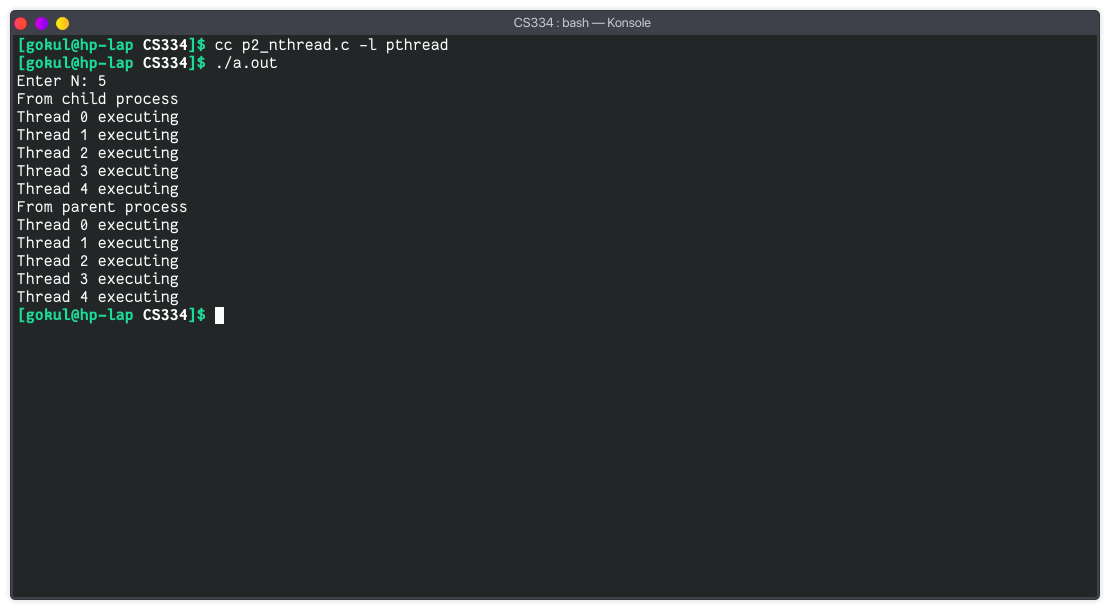
\includegraphics[width=0.90\textwidth]{img/p3.png}
\end{center}

\subsection{Result}
The above program was executed and its output was verified